% 菱形性质：四边相等、对角线垂直平分、平分对角
\documentclass[tikz,border=4pt]{standalone}
\usepackage{ctex}
\usepackage{amsmath}
\usetikzlibrary{calc, decorations.markings}
\begin{document}
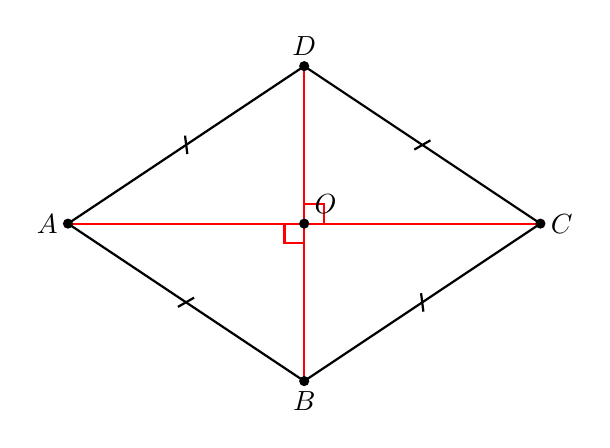
\begin{tikzpicture}[scale=1.0, thick,
  tickone/.style={postaction={decorate, decoration={markings,
    mark=at position 0.5 with {\draw (-1.5pt,-3pt) -- (1.5pt,3pt);}}}},
]
  % 菱形：对角线水平/竖直，中心在原点
  \coordinate (A) at (-3,0);
  \coordinate (B) at (0,-2);
  \coordinate (C) at (3,0);
  \coordinate (D) at (0,2);
  \coordinate (O) at (0,0);
  \draw[tickone] (A) -- (B);
  \draw[tickone] (B) -- (C);
  \draw[tickone] (C) -- (D);
  \draw[tickone] (D) -- (A);
  \draw[red, thick] (A) -- (C);
  \draw[red, thick] (B) -- (D);
  % 直角小方块在 O
  \draw[red] (0.25,0) -- (0.25,0.25) -- (0,0.25);
  \draw[red] (-0.25,0) -- (-0.25,-0.25) -- (0,-0.25);
  \foreach \pt in {A,B,C,D,O} \filldraw (\pt) circle (1.4pt);
  \node[left]  at (A) {$A$};
  \node[below] at (B) {$B$};
  \node[right] at (C) {$C$};
  \node[above] at (D) {$D$};
  \node[above right] at (O) {$O$};
\end{tikzpicture}
\end{document}
